\chapter{Design and Implementation}
\label{chap:Design}

\section{Network Infrastructure}
    \begin{figure}[H]
        \centering
        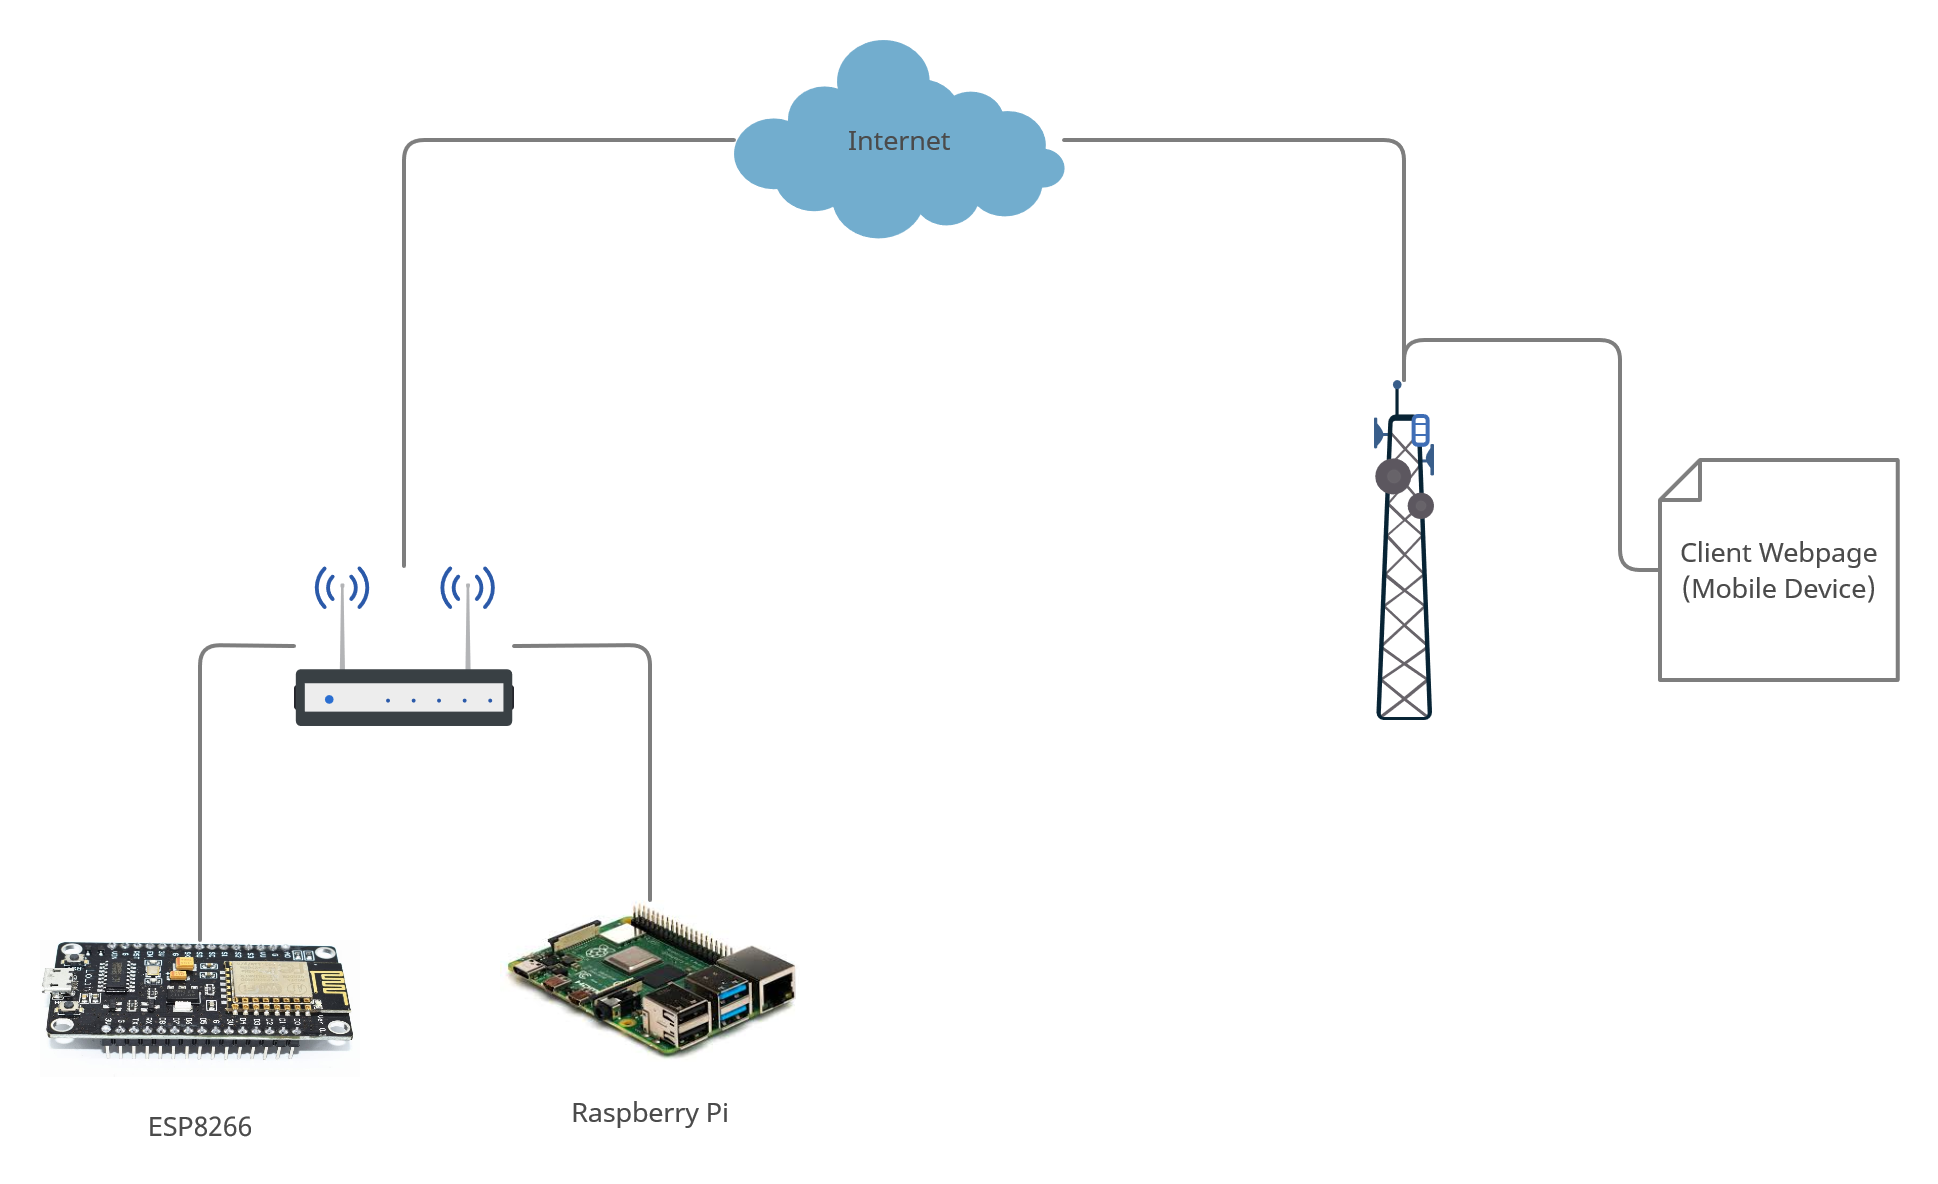
\includegraphics[width=14cm]{images/network.png}
        \caption{Network Infrastructure}
    \end{figure}
    \begin{flushleft}
        The networking layout was designed because it was the most important stack of all. The network infrastructure is not only 
        responsible for connecting the device to one another but also to expose the device to the outside world. The router runs a 
        custom \textbf{OpenWRT} based firmware with a \textbf{Wireguard VPN} service to make sure no one else can access the private
        data from our authentication system. Using \textbf{NAT}, the router merges the private network to the public internet.

        On the client device a \textbf{Wireguard Configuration} will be installed to connect with the private network.
    \end{flushleft}


\section{Intrusion Detection Sensor}
    \begin{figure}[H]
        \centering
        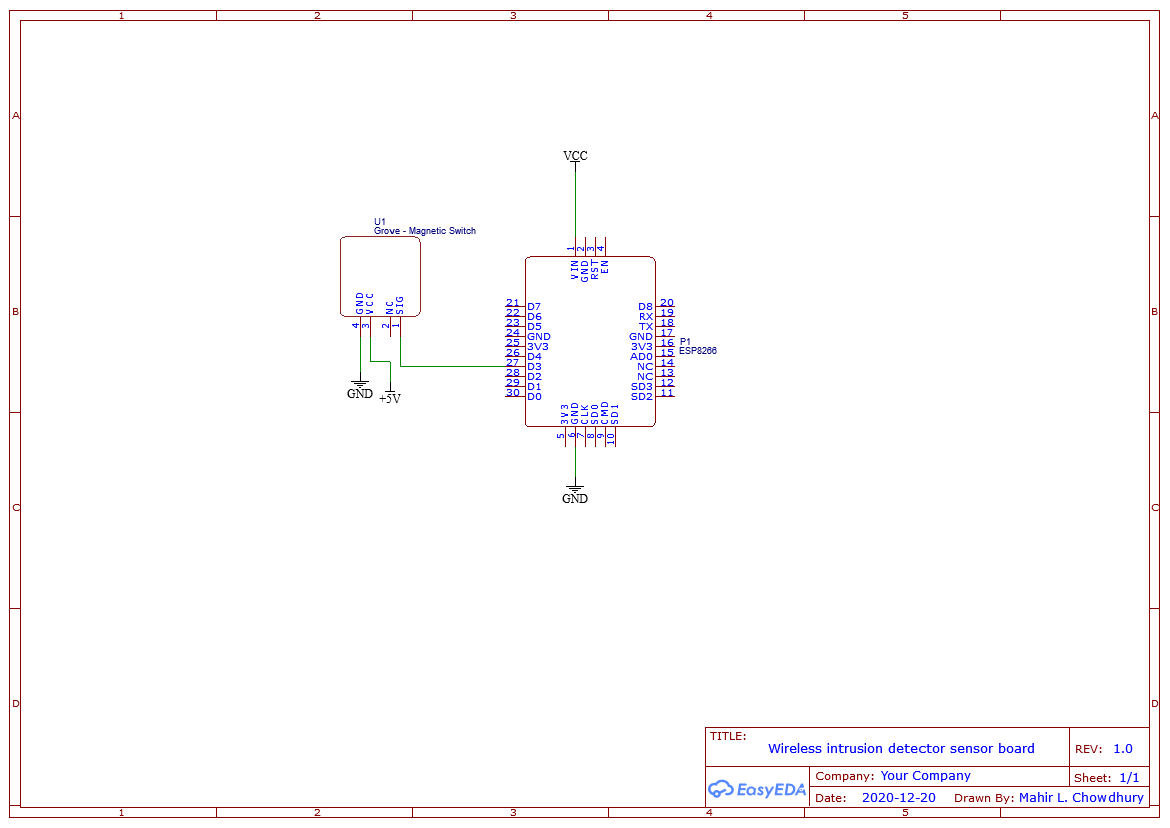
\includegraphics[width=16cm]{images/schematic.png}
        \caption{Schematic of Intrusion Detection Sensor}
    \end{figure}
    \begin{flushleft}
        The intrusion the detection sensor is in reality a very simple device. It uses a magnetic contact switch connected 
        to the ESP8266 and is powered from a 5V wall adapter. When the door/window is opened it senses the change by the switch activating 
        and detecting this change the ESP8266 will send an message to the MQTT broker. The message in the broker is then used to 
        trigger the alert from the authentication server.  
    \end{flushleft}


\section{Authentication Server}
    \begin{flushleft}
        The authentication server is arguably the most important part of this whole project. The server is responsible 
        for the following aspects:
    \end{flushleft}
    \begin{enumerate}
        \item Authorization
        \item Face Recognition
        \item Managing The Camera
        \item Interfacing with The Keypad
        \item Registration of Face Data
        \item Logging of Entry and Exit
        \item Running The Database Server
        \item Sending Alert to The User of Intrusion Detection
        \item Running MQTT broker
    \end{enumerate}
    \subsection{The Functional Blocks of Authentication Server}
    \begin{figure}[H]
        \centering
        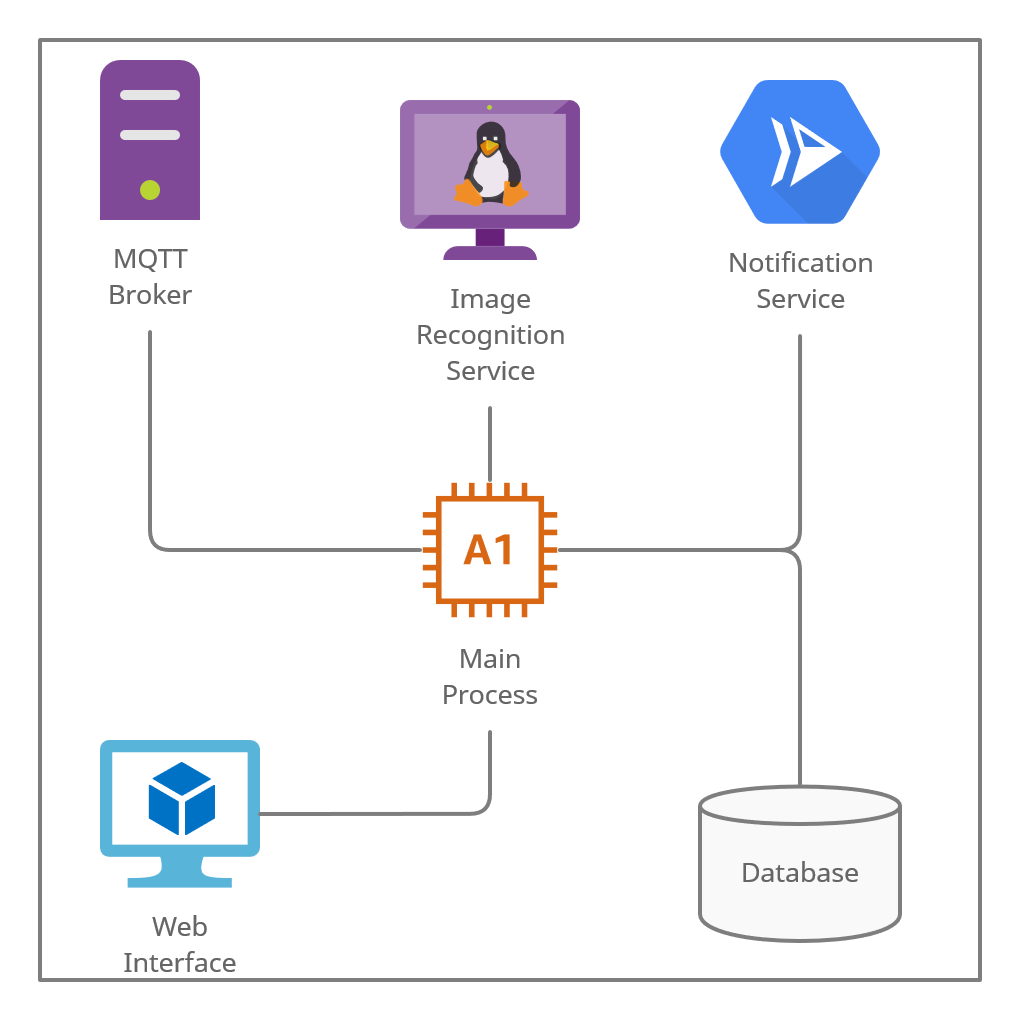
\includegraphics[width=14cm]{images/auth_server.png}
        \caption{Functional Part of Authentication Server}
    \end{figure}
        \subsubsection{Main Process}
        \begin{flushleft}
            The main process ties everything together. It is responsible for managing and interfacing with all the other parts of
            the server.
        \end{flushleft}

        \subsubsection{Image Recognition Service}
        \begin{flushleft}
            This used \textbf{OpenCV} with \textbf{dlib} to recognize faces and check their authorization.
        \end{flushleft}
        \begin{figure}[H]
            \centering
            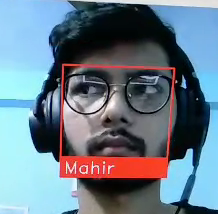
\includegraphics[width=6cm]{images/facerec.png}
            \caption{Demonstrating Facial Recognition Capabilities}
        \end{figure}

        \subsubsection{MQTT Broker}
        \begin{flushleft}
            MQTT Broker is a message queue and broker. It supports very low latency message delivery and a variety of message channels.
            It is used to receive data from the ``Intrusion Detection Sensor'' and send to the Main Process.
        \end{flushleft}

        \subsubsection{Notification Service}
        \begin{flushleft}
            Sends `Push Notification' to the various client devices that are configured to receive. 
        \end{flushleft}

        \subsubsection{Web Interface}
        \begin{flushleft}
            The web interface is used for managing the whole system. It is used to enrol new authorized user to the
            authorization list also to see the log data.
        \end{flushleft}
        \begin{figure}[H]
            \centering
            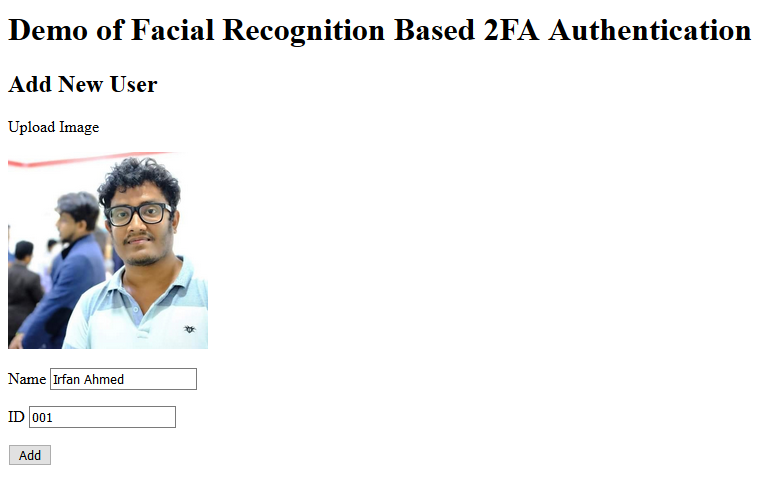
\includegraphics[width=14cm]{images/adduser.png}
            \caption{User Adding Interface}
        \end{figure}

        \begin{figure}[H]
            \centering
            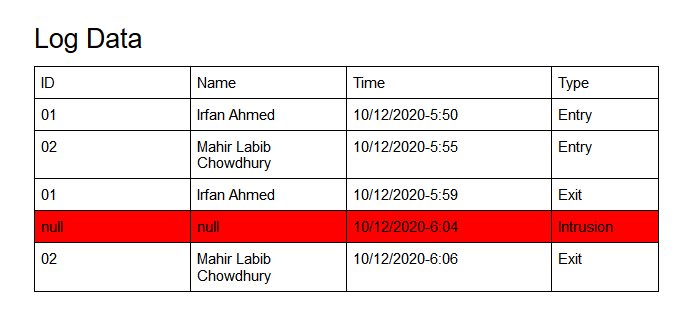
\includegraphics[width=14cm]{images/log.png}
            \caption{Entry/Exit Log }
        \end{figure}

        \subsubsection{Database}
        \begin{flushleft}
            The database is used to keep the time logs. It is running a redis server underneath. So the data is stored 
            in a key-value pair for faster access times and lower latency.
        \end{flushleft}




